% !TEX root = Projektdokumentation.tex

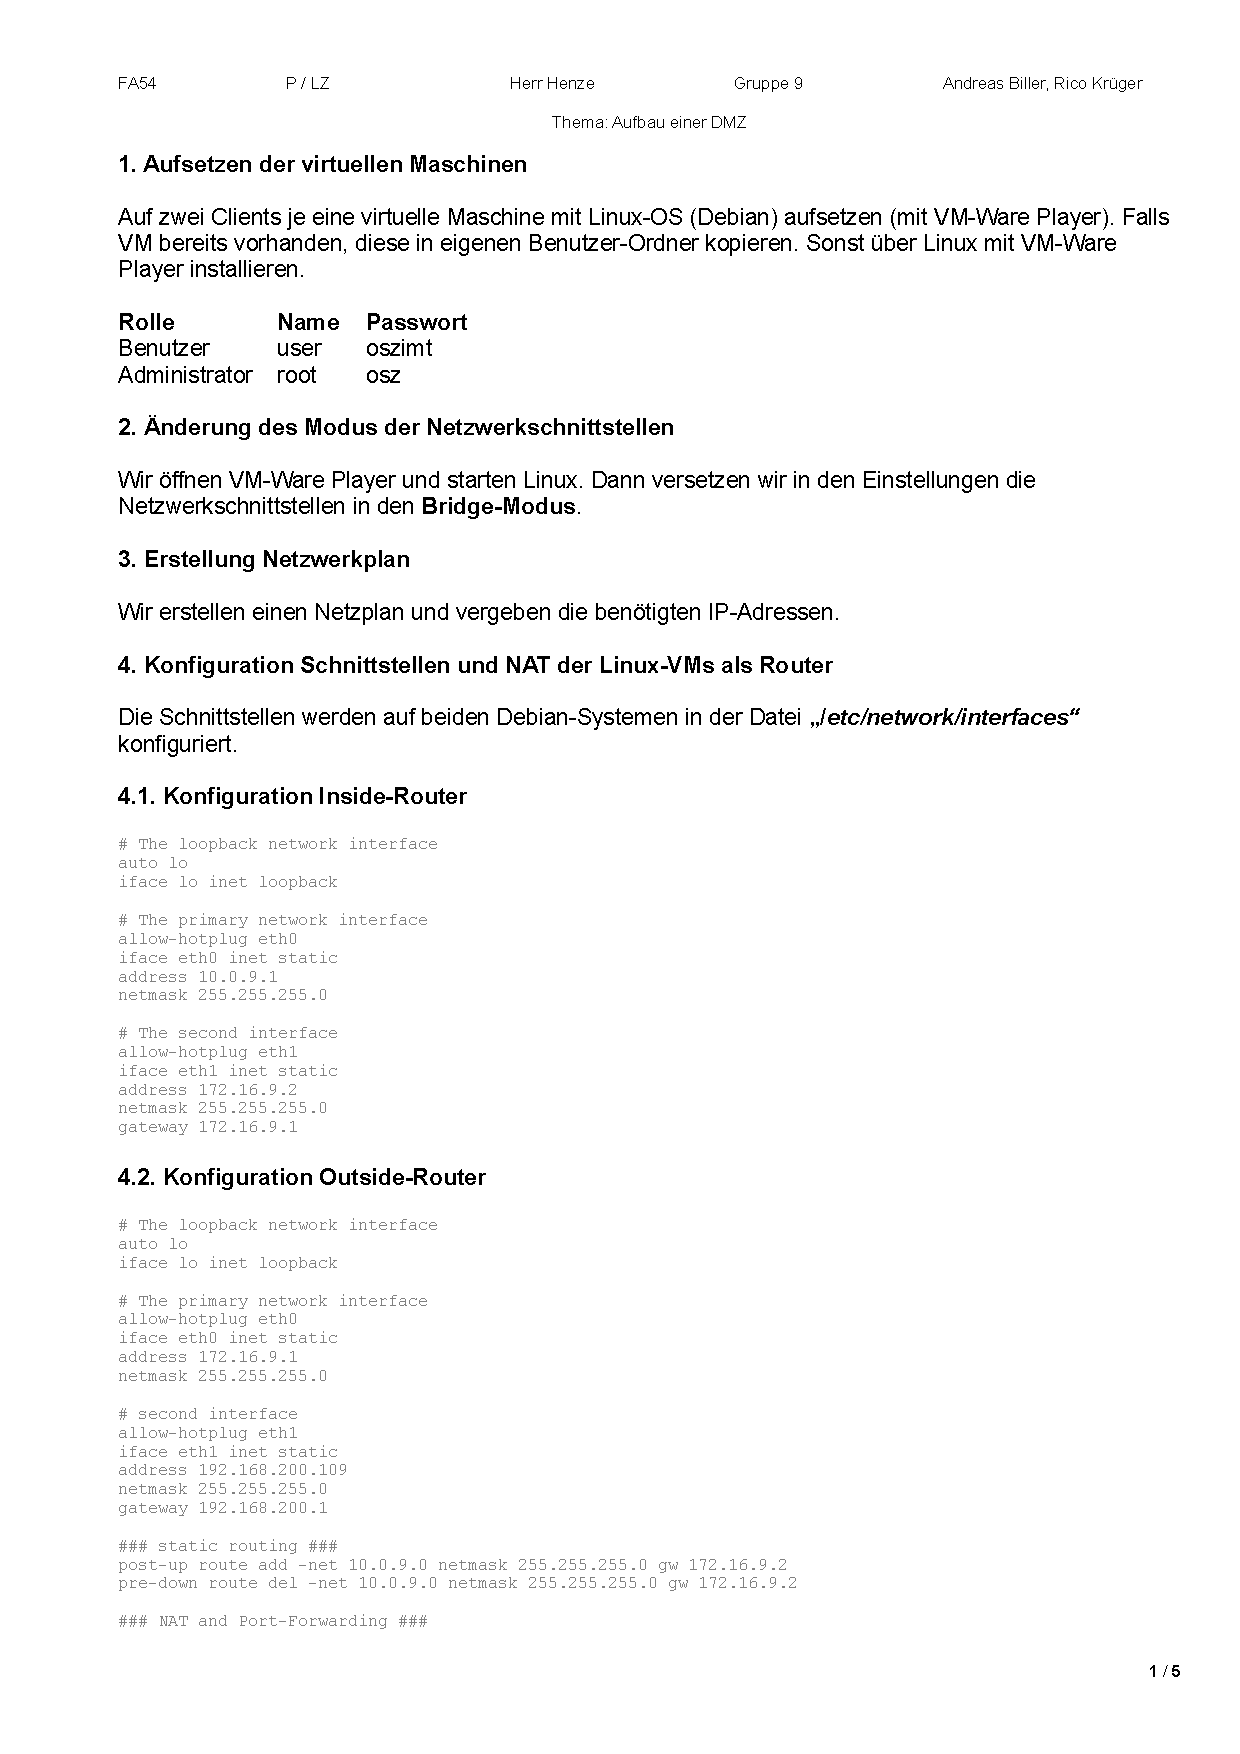
\includepdf[scale=0.8,clip,trim=0cm 0cm 0cm 0cm,offset=0 -2cm,pages={1},pagecommand={\section{Anhang}\subsection{Schritt-für-Schritt Anleitung}\label{app:Anleitung}}]{AufbauEinerDMZ.pdf} \includepdf[scale=0.85,clip,trim=0cm 0cm 0cm 0cm,offset=0 -0.5cm,pages={2-5},pagecommand={}]{AufbauEinerDMZ.pdf}

\subsection{Detaillierte Zeitplanung}
\label{app:Zeitplanung}

\tabelleAnhang{ZeitplanungKomplett}

\subsection{Lastenheft (Auszug)}
\label{app:Lastenheft}
Es folgt ein Auszug aus dem Lastenheft mit Fokus auf die Anforderungen:

Die Anwendung muss folgende Anforderungen erfüllen: 
\begin{enumerate}[itemsep=0em,partopsep=0em,parsep=0em,topsep=0em]
\item Verarbeitung der Moduldaten
	\begin{enumerate}
	\item Die Anwendung muss die von Subversion und einem externen Programm bereitgestellten Informationen (z.B. Source-Benutzer, -Datum, Hash) verarbeiten.
	\item Auslesen der Beschreibung und der Stichwörter aus dem Sourcecode.
	\end{enumerate}
\item Darstellung der Daten
	\begin{enumerate}
	\item Die Anwendung muss eine Liste aller Module erzeugen inkl. Source-Benutzer und -Datum, letztem Commit-Benutzer und -Datum für alle drei Umgebungen. 
	\item Verknüpfen der Module mit externen Tools wie z.B. Wiki-Einträgen zu den Modulen oder dem Sourcecode in Subversion.
	\item Die Sourcen der Umgebungen müssen verglichen und eine schnelle Übersicht zur Einhaltung des allgemeinen Entwicklungsprozesses gegeben werden. 
	\item Dieser Vergleich muss auf die von einem bestimmten Benutzer bearbeiteten Module eingeschränkt werden können. 
	\item Die Anwendung muss in dieser Liste auch Module anzeigen, die nach einer Bearbeitung durch den gesuchten Benutzer durch jemand anderen bearbeitet wurden. 
	\item Abweichungen sollen kenntlich gemacht werden. 
	\item Anzeigen einer Übersichtsseite für ein Modul mit allen relevanten Informationen zu diesem.
	\end{enumerate}
\item Sonstige Anforderungen
	\begin{enumerate}
	\item Die Anwendung muss ohne das Installieren einer zusätzlichen Software über einen Webbrowser im Intranet erreichbar sein.
	\item Die Daten der Anwendung müssen jede Nacht \bzw nach jedem \acs{SVN}-Commit automatisch aktualisiert werden. 
	\item Es muss ermittelt werden, ob Änderungen auf der Produktionsumgebung vorgenommen wurden, die nicht von einer anderen Umgebung kopiert wurden. Diese Modulliste soll als Mahnung per E-Mail an alle Entwickler geschickt werden (Peer Pressure).
	\item Die Anwendung soll jederzeit erreichbar sein.
	\item Da sich die Entwickler auf die Anwendung verlassen, muss diese korrekte Daten liefern und darf keinen Interpretationsspielraum lassen.
	\item Die Anwendung muss so flexibel sein, dass sie bei Änderungen im Entwicklungsprozess einfach angepasst werden kann.
	\end{enumerate}
\end{enumerate}


\clearpage

\subsection{Use Case-Diagramm}
\label{app:UseCase}
Use Case-Diagramme und weitere \acs{UML}-Diagramme kann man auch direkt mit \LaTeX{} zeichnen, siehe \zB \url{http://metauml.sourceforge.net/old/usecase-diagram.html}.
\begin{figure}[htb]
\centering
\includegraphicsKeepAspectRatio{UseCase.pdf}{0.7}
\caption{Use Case-Diagramm}
\end{figure}

\subsection{Pflichtenheft (Auszug)}
\label{app:Pflichtenheft}

\subsubsection*{Zielbestimmung}

\begin{enumerate}[itemsep=0em,partopsep=0em,parsep=0em,topsep=0em]
\item Musskriterien % Wikipedia: für das Produkt unabdingbare Leistungen, die in jedem Fall erfüllt werden müssen
	\begin{enumerate}
	\item Modul-Liste: Zeigt eine filterbare Liste der Module mit den dazugehörigen Kerninformationen sowie Symbolen zur Einhaltung des Entwicklungsprozesses an
		\begin{itemize}
		\item In der Liste wird der Name, die Bibliothek und Daten zum Source und Kompilat eines Moduls angezeigt.
		\item Ebenfalls wird der Status des Moduls hinsichtlich Source und Kompilat angezeigt. Dazu gibt es unterschiedliche Status-Zeichen, welche symbolisieren in wie weit der Entwicklungsprozess eingehalten wurde \bzw welche Schritte als nächstes getan werden müssen. So gibt es \zB Zeichen für das Einhalten oder Verletzen des Prozesses oder den Hinweis auf den nächsten zu tätigenden Schritt. 
		\item Weiterhin werden die Benutzer und Zeitpunkte der aktuellen Version der Sourcen und Kompilate angezeigt. Dazu kann vorher ausgewählt werden, von welcher Umgebung diese Daten gelesen werden sollen. 
		\item Es kann eine Filterung nach allen angezeigten Daten vorgenommen werden. Die Daten zu den Sourcen sind historisiert. Durch die Filterung ist es möglich, auch Module zu finden, die in der Zwischenzeit schon von einem anderen Benutzer editiert wurden.
		\end{itemize}
	\item Tag-Liste: Bietet die Möglichkeit die Module anhand von Tags zu filtern. 
		\begin{itemize}
		\item Es sollen die Tags angezeigt werden, nach denen bereits gefiltert wird und die, die noch der Filterung hinzugefügt werden könnten, ohne dass die Ergebnisliste leer wird.
		\item Zusätzlich sollen die Module angezeigt werden, die den Filterkriterien entsprechen. Sollten die Filterkriterien leer sein, werden nur die Module angezeigt, welche mit einem Tag versehen sind.
		\end{itemize}
	\item Import der Moduldaten aus einer bereitgestellten \acs{CSV}-Datei
		\begin{itemize}
		\item Es wird täglich eine Datei mit den Daten der aktuellen Module erstellt. Diese Datei wird (durch einen Cronjob) automatisch nachts importiert.
		\item Dabei wird für jedes importierte Modul ein Zeitstempel aktualisiert, damit festgestellt werden kann, wenn ein Modul gelöscht wurde.
		\item Die Datei enthält die Namen der Umgebung, der Bibliothek und des Moduls, den Programmtyp, den Benutzer und Zeitpunkt des Sourcecodes sowie des Kompilats und den Hash des Sourcecodes.
		\item Sollte sich ein Modul verändert haben, werden die entsprechenden Daten in der Datenbank aktualisiert. Die Veränderungen am Source werden dabei aber nicht ersetzt, sondern historisiert.
		\end{itemize}
	\item Import der Informationen aus \ac{SVN}. Durch einen \gqq{post-commit-hook} wird nach jedem Einchecken eines Moduls ein \acs{PHP}-Script auf der Konsole aufgerufen, welches die Informationen, die vom \ac{SVN}-Kommandozeilentool geliefert werden, an \acs{NatInfo} übergibt.
	\item Parsen der Sourcen
		\begin{itemize}
		\item Die Sourcen der Entwicklungsumgebung werden nach Tags, Links zu Artikeln im Wiki und Programmbeschreibungen durchsucht.
		\item Diese Daten werden dann entsprechend angelegt, aktualisiert oder nicht mehr gesetzte Tags/Wikiartikel entfernt.
		\end{itemize}
	\item Sonstiges
		\begin{itemize}
		\item Das Programm läuft als Webanwendung im Intranet.
		\item Die Anwendung soll möglichst leicht erweiterbar sein und auch von anderen Entwicklungsprozessen ausgehen können.
		\item Eine Konfiguration soll möglichst in zentralen Konfigurationsdateien erfolgen.
		\end{itemize}
	\end{enumerate}
\end{enumerate}

\subsubsection*{Produkteinsatz}

\begin{enumerate}[itemsep=0em,partopsep=0em,parsep=0em,topsep=0em]
\item{Anwendungsbereiche\\
Die Webanwendung dient als Anlaufstelle für die Entwicklung. Dort sind alle Informationen für die Module an einer Stelle gesammelt. Vorher getrennte Anwendungen werden ersetzt \bzw verlinkt.}
\item{Zielgruppen\\
\NI wird lediglich von den \ac{Natural}-Entwicklern in der EDV-Abteilung genutzt.}
\item{Betriebsbedingungen\\ % Wikipedia: physikalische Umgebung des Systems, tägliche Betriebszeit, ständige Beobachtung des Systems durch Bediener oder unbeaufsichtigter Betrieb
Die nötigen Betriebsbedingungen, also der Webserver, die Datenbank, die Versionsverwaltung, das Wiki und der nächtliche Export sind bereits vorhanden und konfiguriert. Durch einen täglichen Cronjob werden entsprechende Daten aktualisiert, die Webanwendung ist jederzeit aus dem Intranet heraus erreichbar.}
\end{enumerate}


\subsection{Netzplan}
\label{app:Netzplan}
Der Netzplan unserer \acs{DMZ}
\begin{figure}[htb]
\centering
\includegraphicsKeepAspectRatio{PLZNetzplanProjektumgebung.png}{1}
\caption{Netzplan der DMZ (Arbeitsgruppe 9)}
\end{figure}
\clearpage

\subsection{Oberflächenentwürfe}
\label{app:Entwuerfe}
\begin{figure}[htb]
\centering
\includegraphicsKeepAspectRatio{MockupModules.pdf}{0.7}
\caption{Liste der Module mit Filtermöglichkeiten}
\end{figure}

\begin{figure}[htb]
\centering
\includegraphicsKeepAspectRatio{MockupModul.pdf}{0.7}
\caption{Anzeige der Übersichtsseite einzelner Module}
\end{figure}

\begin{figure}[htb]
\centering
\includegraphicsKeepAspectRatio{MockupTag.pdf}{0.7}
\caption{Anzeige und Filterung der Module nach Tags}
\end{figure}

\clearpage
\subsection{Screenshots der Anwendung}
\label{Screenshots}
\begin{figure}[htb]
\centering
\includegraphicsKeepAspectRatio{tagliste.pdf}{1}
\caption{Anzeige und Filterung der Module nach Tags}
\end{figure}
\clearpage
\begin{figure}[htb]
\centering
\includegraphicsKeepAspectRatio{modulliste.pdf}{1}
\caption{Liste der Module mit Filtermöglichkeiten}
\end{figure}
\clearpage

\subsection{Entwicklerdokumentation}
\label{app:Doc}
\begin{center}
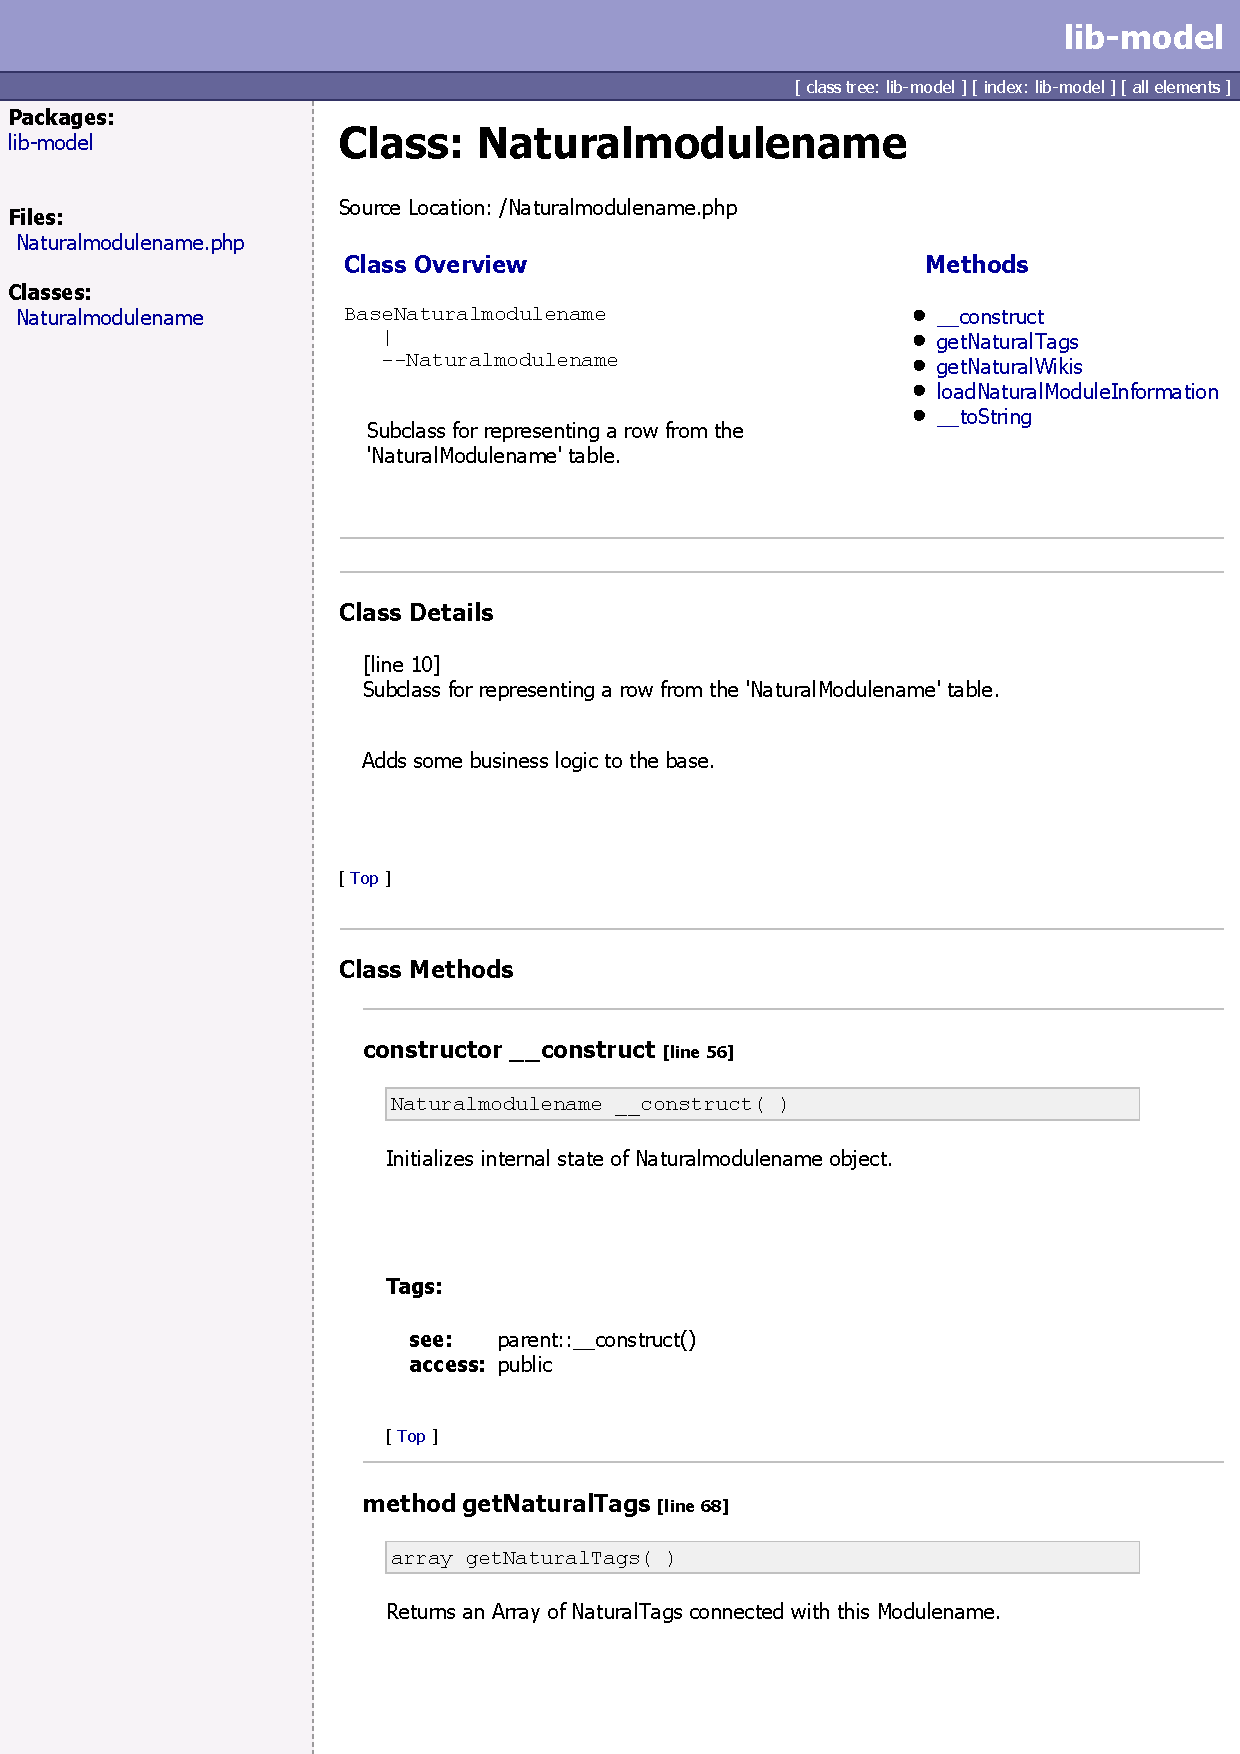
\includegraphics[page=1, width=0.9\textwidth]{doc.pdf}

\includegraphics[page=2, width=0.9\textwidth]{doc.pdf}
\end{center}

\clearpage
\begin{table}
    \tabelleAnhang{Systeminformation}{tab:Systeminformation}{Systeminformation.tex}
    \caption{Hardwaredetails des Testsystems}
    \label{tab:tabletestsystem}
\end{table}

\subsection{Aufbau der Testumgebung}
\label{app:testaufbau}
Die zur Umsetzung dieses Kapitels benötigten Informationen entstammen unter anderem den hilfreichen Artikeln folgender Webseiten: \cite{networkdriverhacking}

\subsubsection{Implementierung der Virtuellen Maschinen}
Im Server-Manager fügen wir über \textit{Verwalten > Rollen und Features hinzufügen} den Hyper-V-Manager hinzu indem wir dem Assistenten folgen. Dieser gestattet es virtuelle Maschinen und Netzwerke zu installieren.
Als nächstes wird eine neue virtuelle Linux (Debian 7.1)  Maschine (Generation 1) aus einem Image erstellt. Dies geschieht mit Hilfe eines Assistenten. Sie bekommt einen virtuellen Prozessor und 1 \ac{GB} Arbeitsspeicher. Des weiteren wird bei der Installation eine 5 \ac{GB} große Festplatte für die Maschine erstellt und ihr zugewiesen. Als virtuellen Switch weisen wir ihr vorläufig den Netzwerkadapter des Hosts zu. Somit besitzt unsere Linux-\ac{VM} Internet. Um sie zu installieren, startet man nun die Maschine und verbindet sich zu ihr. Danach folgt man wie gewohnt den Installationsschritten wie bei einer physischen Maschine. Danach installieren wir den \ac{NTP}-Service. Ist die Grundkonfiguration fertig, wird die Maschine ausgeschaltet.
Die Installation der Windows 7 \ac{VM} erfolgt analog zu die der Linux \ac{VM}. Wir vergeben jedoch 4 \ac{GB} \ac{RAM} und erstellen eine mindestens 30 \ac{GB} große virtuelle Festplatte. Nach der Installation wird die Firewall wie in \nameref{sec:Implementierungsphase} eingerichtet. Zusätzlich werden noch nützliche Software wie putty oder winscp heruntergeladen.
Nach der Grundkonfiguration der beiden \ac{VM}s können diese nun dupliziert werden. Dazu muss man die virtuelle Maschine erst exportieren, um sie danach wieder zu importieren. Beim Import sollte man darauf achten, dass man \textit{eine neue eindeutige \ac{ID} } erstellt. Nachdem starten der importierten Maschine wird als erstes der Hostname geändert, um sie von der Originalen zu unterscheiden und um \ac{DNS}-Konflikte zu vermeiden.

\subsubsection{Implementierung des virtuellen Netzwerkes}
Virtuelle Netzwerke werden über das Hinzufügen virtueller Switche an den Netzwerkadaptern der virtuellen Maschine erstellt. Auf diesen lassen sich auch \ac{VLAN}s einrichten.
Die Installation eines solchen Switch wird ebenfalls vom Hyper-V-Manager mit einem Assistenten bereitgestellt. Für Testzwecke werden 2 \textit{private} Switche erstellt, da diese die direkte Kommunikation mit dem Host unterbinden und somit nicht die Router umgangen werden. Diese erhalten den Namen \ac{DMZ}- \bzw \ac{LAN}-Switch. Ein \textit{öffentlicher} Switch ist bereits vorhanden. Mit diesem ist der physische Netzwerkadapter des Hosts verbunden. Diese werden dann den \ac{VM}s entsprechend des \nameref{app:Netzplan}s zugeordnet. Für die Linux-\ac{VM}s, die als Router fungieren, muss \evtl noch ein zweiter Netzwerkadapter hinzugefügt werden. Nun können die Router und Clients (\text{Siehe Bild und Implementierung}) konfiguriert werden.

\subsubsection{Implementierung des \ac{DNS}-Servers}
Der \ac{DNS}-Server wird ebenfalls über den Server-Manager (unter \textit{Rollen und Features hinzufügen}) installiert. Diesen kann man nun über den \ac{DNS}-Manager verwalten. Es genügt eine \textit{Forward-Lookup}-Zone zu erstellen. Als Zonennamen wählen wir \textit{fritz.box} da bereits das Standard-Gateway darauf verweist. Dies ist die Domäne bzw. das \ac{DNS}-Suffix. Dieses Suffix wird auf den Windows-\ac{VM}s in den \ac{IP}v4-Einstellungen des Netzwerkadapters nachgetragen. Auf den Linux-\ac{VM}s tragen wir dies zusätzlich in die \verb+/etc/resolv.conf+ vor unserem \ac{DNS}-Server ein. \textbf{siehe resolv.conf oder selber schreiben]
Über den \ac{DNS}-Manager werden im Anschluss noch in der Zone \textit{fritz.box} unsere \ac{VM}s (A-Record) mit Namen und \ac{IP}-Adressen eingetragen. \textbf Siehe \ac{DNS}Manager.png}.

\subsubsection{Testen der Firewall}
Nachdem das Firewall-Script auf die Router kopiert und die \ac{DNS}-Server angepasst wurden, kann mit den Tests begonnen und die Firewall ggf.\ angepasst werden. Dazu speichern wir den Verlauf der erstellten Regeln als Log-Ausgabe in \verb+/var/log/firewall/firewallConfig+ ab. Die Ergebnisse unserer Tests finden sich als Übersicht in den folgenden Tabellen der Testprotokolle:


% Testprotokolle
\subsubsection{Testprotokolle}
\label{app:Testprotokolle}
% Description
\clearpage

% tables created with: http://www.tablesgenerator.com/latex_tables
% Please add the following required packages to your document preamble:
% \usepackage{graphicx}
% \usepackage[table,xcdraw]{xcolor}
% If you use beamer only pass "xcolor=table" option, i.e. \documentclass[xcolor=table]{beamer}
\begin{table}[]
    \resizebox{\textwidth}{!}{%
        \begin{tabular}{llllll}
            \rowcolor[HTML]{009BA7} 
            \textbf{Service} & \textbf{Command} & \textbf{Source-IP} & \textbf{Destination-IP} & \textbf{Soll} & \textbf{Ist} \\
            ICMP & ping & 10.0.9.2 & 10.0.9.1 & ja & ja \\
            \rowcolor[HTML]{EFEFEF} 
            ICMP & ping & 10.0.9.3 & 10.0.9.1 & ja & ja \\
            ICMP & ping & 10.0.9.2 & 172.16.9.1 & ja & ja \\
            \rowcolor[HTML]{EFEFEF} 
            ICMP & ping & 10.0.9.3 & 172.16.9.1 & ja & ja \\
            ICMP & ping & 172.16.9.3 & 172.16.9.1 & ja & ja \\
            \rowcolor[HTML]{EFEFEF} 
            ICMP & ping & 172.16.9.3 & 172.16.9.2 & ja & ja \\
            ICMP & ping & 10.0.9.3 & 192.168.200.10 & ja & ja \\
            \rowcolor[HTML]{EFEFEF} 
            ICMP & ping & 192.168.200.10 & 10.0.9.3 & ja & ja \\
            ICMP & ping & 192.168.200.10 & 172.16.9.3 & ja & ja \\
            \rowcolor[HTML]{EFEFEF} 
            ICMP & ping & 192.168.200.10 & 192.168.200.109 & ja & ja \\
            ICMP & ping & 10.0.9.3 & 8.8.8.8 & ja & ja \\
            \rowcolor[HTML]{EFEFEF} 
            HTTP & http://172.16.9.3 & 192.168.200.10 & 192.168.200.109 & ja & ja \\
            HTTP & http://172.16.9.3 & 192.168.200.10 & 172.16.9.3 & ja & ja \\
            \rowcolor[HTML]{EFEFEF} 
            HTTP & http://172.16.9.3 & 10.0.9.3 & 192.168.200.109 & ja & ja \\
            HTTP & http://172.16.9.3 & 10.0.9.3 & 172.16.9.3 & ja & ja \\
            \rowcolor[HTML]{EFEFEF} 
            NTP & w32tm /stripchart /computer:192.168.200.1 & 10.0.9.2 & 192.168.200.1 & ja & ja \\
            NTP & w32tm /stripchart /computer:192.168.200.1 & 172.16.9.3 & 192.168.200.1 & ja & ja \\
            \rowcolor[HTML]{EFEFEF} 
            NTP & ntpq -p & 192.168.200.109 & 192.168.200.1 & ja & ja \\
            RDP & mstsc.exe & 10.0.9.2 & 172.16.9.3 & ja & ja \\
            \rowcolor[HTML]{EFEFEF} 
            RDP & mstsc.exe & 10.0.9.3 & 172.16.9.3 & ja & ja \\
            SSH & putty & 10.0.9.2 & 10.0.9.1 & ja & ja \\
            \rowcolor[HTML]{EFEFEF} 
            SSH & putty & 10.0.9.2 & 172.16.9.1 & ja & ja \\
            SSH & putty & 10.0.9.3 & 10.0.9.1 & ja & ja \\
            \rowcolor[HTML]{EFEFEF} 
            SSH & putty & 10.0.9.3 & 172.16.9.1 & ja & ja \\
            SSH & putty & 172.16.9.3 & 172.16.9.1 & ja & ja \\
            \rowcolor[HTML]{EFEFEF} 
            SSH & putty & 172.16.9.3 & 172.16.9.2 & ja & ja \\
            DNS & nslookup 172.16.9.1 & 10.0.9.3 & 192.168.200.10 & ja & ja \\
            \rowcolor[HTML]{EFEFEF} 
            DNS & nslookup Inside-Router & 172.16.9.3 & 192.168.200.10 & ja & ja \\
            DNS & nslookup 10.0.9.1 & 172.16.9.2 & 192.168.200.10 & ja & ja \\
            \rowcolor[HTML]{EFEFEF} 
            DNS & nslookup Client-PC & 192.168.200.109 & 192.168.200.10 & ja & ja
        \end{tabular}%
    }
    \caption{Aus - Aus}
    \label{tab:ausaus}
\end{table}

% Please add the following required packages to your document preamble:
% \usepackage{graphicx}
% \usepackage[table,xcdraw]{xcolor}
% If you use beamer only pass "xcolor=table" option, i.e. \documentclass[xcolor=table]{beamer}
\begin{table}[]
    \resizebox{\textwidth}{!}{%
        \begin{tabular}{llllll}
            \rowcolor[HTML]{009BA7} 
            \textbf{Service} & \textbf{Command} & \textbf{Source-IP} & \textbf{Destination-IP} & \textbf{Soll} & \textbf{Ist} \\
            ICMP & ping & 10.0.9.2 & 10.0.9.1 & ja & ja \\
            \rowcolor[HTML]{EFEFEF} 
            ICMP & ping & 10.0.9.3 & 10.0.9.1 & nein & nein \\
            ICMP & ping & 10.0.9.2 & 172.16.9.1 & ja & ja \\
            \rowcolor[HTML]{EFEFEF} 
            ICMP & ping & 10.0.9.3 & 172.16.9.1 & nein & nein \\
            ICMP & ping & 172.16.9.3 & 172.16.9.1 & ja & ja \\
            \rowcolor[HTML]{EFEFEF} 
            ICMP & ping & 172.16.9.3 & 172.16.9.2 & nein & nein \\
            ICMP & ping & 10.0.9.3 & 192.168.200.10 & ja & ja \\
            \rowcolor[HTML]{EFEFEF} 
            ICMP & ping & 192.168.200.10 & 10.0.9.3 & nein & nein \\
            ICMP & ping & 192.168.200.10 & 172.16.9.3 & ja & ja \\
            \rowcolor[HTML]{EFEFEF} 
            ICMP & ping & 192.168.200.10 & 192.168.200.109 & ja & ja \\
            ICMP & ping & 10.0.9.3 & 8.8.8.8 & ja & ja \\
            \rowcolor[HTML]{EFEFEF} 
            HTTP & http://172.16.9.3 & 192.168.200.10 & 192.168.200.109 & ja & ja \\
            HTTP & http://172.16.9.3 & 192.168.200.10 & 172.16.9.3 & ja & ja \\
            \rowcolor[HTML]{EFEFEF} 
            HTTP & http://172.16.9.3 & 10.0.9.3 & 192.168.200.109 & nein & nein \\
            HTTP & http://172.16.9.3 & 10.0.9.3 & 172.16.9.3 & ja & ja \\
            \rowcolor[HTML]{EFEFEF} 
            NTP & w32tm /stripchart /computer:192.168.200.1 & 10.0.9.2 & 192.168.200.1 & ja & ja \\
            NTP & w32tm /stripchart /computer:192.168.200.1 & 172.16.9.3 & 192.168.200.1 & ja & ja \\
            \rowcolor[HTML]{EFEFEF} 
            NTP & ntpq -p & 192.168.200.109 & 192.168.200.1 & ja & ja \\
            RDP & mstsc.exe & 10.0.9.2 & 172.16.9.3 & ja & ja \\
            \rowcolor[HTML]{EFEFEF} 
            RDP & mstsc.exe & 10.0.9.3 & 172.16.9.3 & nein & nein \\
            SSH & putty & 10.0.9.2 & 10.0.9.1 & ja & ja \\
            \rowcolor[HTML]{EFEFEF} 
            SSH & putty & 10.0.9.2 & 172.16.9.1 & ja & ja \\
            SSH & putty & 10.0.9.3 & 10.0.9.1 & nein & nein \\
            \rowcolor[HTML]{EFEFEF} 
            SSH & putty & 10.0.9.3 & 172.16.9.1 & ja & ja \\
            SSH & putty & 172.16.9.3 & 172.16.9.1 & ja & ja \\
            \rowcolor[HTML]{EFEFEF} 
            SSH & putty & 172.16.9.3 & 172.16.9.2 & nein & nein \\
            DNS & nslookup 172.16.9.1 & 10.0.9.3 & 192.168.200.10 & ja & ja \\
            \rowcolor[HTML]{EFEFEF} 
            DNS & nslookup Inside-Router & 172.16.9.3 & 192.168.200.10 & ja & ja \\
            DNS & nslookup 10.0.9.1 & 172.16.9.2 & 192.168.200.10 & ja & ja \\
            \rowcolor[HTML]{EFEFEF} 
            DNS & nslookup Client-PC & 192.168.200.109 & 192.168.200.10 & ja & ja
        \end{tabular}%
    }
    \caption{Aus - An}
    \label{tab:ausan}
\end{table}

% Please add the following required packages to your document preamble:
% \usepackage{graphicx}
% \usepackage[table,xcdraw]{xcolor}
% If you use beamer only pass "xcolor=table" option, i.e. \documentclass[xcolor=table]{beamer}
\begin{table}[]
    \resizebox{\textwidth}{!}{%
        \begin{tabular}{llllll}
            \rowcolor[HTML]{009BA7} 
            \textbf{Service} & \textbf{Command} & \textbf{Source-IP} & \textbf{Destination-IP} & \textbf{Soll} & \textbf{Ist} \\
            ICMP & ping & 10.0.9.2 & 10.0.9.1 & ja & ja \\
            \rowcolor[HTML]{EFEFEF} 
            ICMP & ping & 10.0.9.3 & 10.0.9.1 & ja & ja \\
            ICMP & ping & 10.0.9.2 & 172.16.9.1 & ja & ja \\
            \rowcolor[HTML]{EFEFEF} 
            ICMP & ping & 10.0.9.3 & 172.16.9.1 & nein & nein \\
            ICMP & ping & 172.16.9.3 & 172.16.9.1 & nein & nein \\
            \rowcolor[HTML]{EFEFEF} 
            ICMP & ping & 172.16.9.3 & 172.16.9.2 & ja & ja \\
            ICMP & ping & 10.0.9.3 & 192.168.200.10 & ja & ja \\
            \rowcolor[HTML]{EFEFEF} 
            ICMP & ping & 192.168.200.10 & 10.0.9.3 & nein & nein \\
            ICMP & ping & 192.168.200.10 & 172.16.9.3 & nein & nein \\
            \rowcolor[HTML]{EFEFEF} 
            ICMP & ping & 192.168.200.10 & 192.168.200.109 & nein & nein \\
            ICMP & ping & 10.0.9.3 & 8.8.8.8 & ja & ja \\
            \rowcolor[HTML]{EFEFEF} 
            HTTP & http://172.16.9.3 & 192.168.200.10 & 192.168.200.109 & ja & ja \\
            HTTP & http://172.16.9.3 & 192.168.200.10 & 172.16.9.3 & ja & ja \\
            \rowcolor[HTML]{EFEFEF} 
            HTTP & http://172.16.9.3 & 10.0.9.3 & 192.168.200.109 & nein & nein \\
            HTTP & http://172.16.9.3 & 10.0.9.3 & 172.16.9.3 & ja & ja \\
            \rowcolor[HTML]{EFEFEF} 
            NTP & w32tm /stripchart /computer:192.168.200.1 & 10.0.9.2 & 192.168.200.1 & ja & ja \\
            NTP & w32tm /stripchart /computer:192.168.200.1 & 172.16.9.3 & 192.168.200.1 & ja & ja \\
            \rowcolor[HTML]{EFEFEF} 
            NTP & ntpq -p & 192.168.200.109 & 192.168.200.1 & ja & ja \\
            RDP & mstsc.exe & 10.0.9.2 & 172.16.9.3 & ja & ja \\
            \rowcolor[HTML]{EFEFEF} 
            RDP & mstsc.exe & 10.0.9.3 & 172.16.9.3 & nein & nein \\
            SSH & putty & 10.0.9.2 & 10.0.9.1 & ja & ja \\
            \rowcolor[HTML]{EFEFEF} 
            SSH & putty & 10.0.9.2 & 172.16.9.1 & ja & ja \\
            SSH & putty & 10.0.9.3 & 10.0.9.1 & ja & ja \\
            \rowcolor[HTML]{EFEFEF} 
            SSH & putty & 10.0.9.3 & 172.16.9.1 & ja & ja \\
            SSH & putty & 172.16.9.3 & 172.16.9.1 & nein & nein \\
            \rowcolor[HTML]{EFEFEF} 
            SSH & putty & 172.16.9.3 & 172.16.9.2 & ja & ja \\
            DNS & nslookup 172.16.9.1 & 10.0.9.3 & 192.168.200.10 & ja & ja \\
            \rowcolor[HTML]{EFEFEF} 
            DNS & nslookup Inside-Router & 172.16.9.3 & 192.168.200.10 & ja & ja \\
            DNS & nslookup 10.0.9.1 & 172.16.9.2 & 192.168.200.10 & ja & ja \\
            \rowcolor[HTML]{EFEFEF} 
            DNS & nslookup Client-PC & 192.168.200.109 & 192.168.200.10 & ja & ja
        \end{tabular}%
    }
    \caption{An - Aus}
    \label{tab:anaus}
\end{table}

% Please add the following required packages to your document preamble:
% \usepackage{graphicx}
% \usepackage[table,xcdraw]{xcolor}
% If you use beamer only pass "xcolor=table" option, i.e. \documentclass[xcolor=table]{beamer}
\begin{table}[]
    \resizebox{\textwidth}{!}{%
        \begin{tabular}{llllll}
            \rowcolor[HTML]{009BA7} 
            \textbf{Service} & \textbf{Command} & \textbf{Source-IP} & \textbf{Destination-IP} & \textbf{Soll} & \textbf{Ist} \\
            ICMP & ping & 10.0.9.2 & 10.0.9.1 & ja & ja \\
            \rowcolor[HTML]{EFEFEF} 
            ICMP & ping & 10.0.9.3 & 10.0.9.1 & ja & ja \\
            ICMP & ping & 10.0.9.2 & 172.16.9.1 & ja & ja \\
            \rowcolor[HTML]{EFEFEF} 
            ICMP & ping & 10.0.9.3 & 172.16.9.1 & nein & nein \\
            ICMP & ping & 172.16.9.3 & 172.16.9.1 & nein & nein \\
            \rowcolor[HTML]{EFEFEF} 
            ICMP & ping & 172.16.9.3 & 172.16.9.2 & ja & ja \\
            ICMP & ping & 10.0.9.3 & 192.168.200.10 & ja & ja \\
            \rowcolor[HTML]{EFEFEF} 
            ICMP & ping & 192.168.200.10 & 10.0.9.3 & nein & nein \\
            ICMP & ping & 192.168.200.10 & 172.16.9.3 & nein & nein \\
            \rowcolor[HTML]{EFEFEF} 
            ICMP & ping & 192.168.200.10 & 192.168.200.109 & nein & nein \\
            ICMP & ping & 10.0.9.3 & 8.8.8.8 & ja & ja \\
            \rowcolor[HTML]{EFEFEF} 
            HTTP & http://172.16.9.3 & 192.168.200.10 & 192.168.200.109 & ja & ja \\
            HTTP & http://172.16.9.3 & 192.168.200.10 & 172.16.9.3 & ja & ja \\
            \rowcolor[HTML]{EFEFEF} 
            HTTP & http://172.16.9.3 & 10.0.9.3 & 192.168.200.109 & nein & nein \\
            HTTP & http://172.16.9.3 & 10.0.9.3 & 172.16.9.3 & ja & ja \\
            \rowcolor[HTML]{EFEFEF} 
            NTP & w32tm /stripchart /computer:192.168.200.1 & 10.0.9.2 & 192.168.200.1 & ja & ja \\
            NTP & w32tm /stripchart /computer:192.168.200.1 & 172.16.9.3 & 192.168.200.1 & ja & ja \\
            \rowcolor[HTML]{EFEFEF} 
            NTP & ntpq -p & 192.168.200.109 & 192.168.200.1 & ja & ja \\
            RDP & mstsc.exe & 10.0.9.2 & 172.16.9.3 & ja & ja \\
            \rowcolor[HTML]{EFEFEF} 
            RDP & mstsc.exe & 10.0.9.3 & 172.16.9.3 & nein & nein \\
            SSH & putty & 10.0.9.2 & 10.0.9.1 & ja & ja \\
            \rowcolor[HTML]{EFEFEF} 
            SSH & putty & 10.0.9.2 & 172.16.9.1 & ja & ja \\
            SSH & putty & 10.0.9.3 & 10.0.9.1 & ja & ja \\
            \rowcolor[HTML]{EFEFEF} 
            SSH & putty & 10.0.9.3 & 172.16.9.1 & ja & ja \\
            SSH & putty & 172.16.9.3 & 172.16.9.1 & nein & nein \\
            \rowcolor[HTML]{EFEFEF} 
            SSH & putty & 172.16.9.3 & 172.16.9.2 & ja & ja \\
            DNS & nslookup 172.16.9.1 & 10.0.9.3 & 192.168.200.10 & ja & ja \\
            \rowcolor[HTML]{EFEFEF} 
            DNS & nslookup Inside-Router & 172.16.9.3 & 192.168.200.10 & ja & ja \\
            DNS & nslookup 10.0.9.1 & 172.16.9.2 & 192.168.200.10 & ja & ja \\
            \rowcolor[HTML]{EFEFEF} 
            DNS & nslookup Client-PC & 192.168.200.109 & 192.168.200.10 & ja & ja
        \end{tabular}%
    }
    \caption{An - An}
    \label{tab:anan}
\end{table}
\clearpage

\subsection{Firewall-Skripte}
\label{app:Firewall}

\subsubsection{firewall.sh (auf dem Outside-Router)}
\label{app:Firewall-Outside}
\lstinputlisting[language=sh]{Listings/outside/firewall.sh}

\subsubsection{firewall.sh (auf dem Inside-Router)}
\label{app:Firewall-Inside}
\lstinputlisting[language=sh]{Listings/inside/firewall.sh}


\subsection{Klasse: ComparedNaturalModuleInformation}
\label{app:CNMI}
Kommentare und simple Getter/Setter werden nicht angezeigt.
\lstinputlisting[language=php]{Listings/cnmi.php}
\clearpage

\subsection{Klassendiagramm}
\label{app:Klassendiagramm}
Klassendiagramme und weitere \acs{UML}-Diagramme kann man auch direkt mit \LaTeX{} zeichnen, siehe \zB \url{http://metauml.sourceforge.net/old/class-diagram.html}.
\begin{figure}[htb]
\centering
\includegraphicsKeepAspectRatio{Klassendiagramm.pdf}{1}
\caption{Klassendiagramm}
\end{figure}
\clearpage

\subsection{Benutzerdokumentation}
\label{app:BenutzerDoku}
Ausschnitt aus der Benutzerdokumentation:

\begin{table}[htb]
\begin{tabularx}{\textwidth}{cXX}
\rowcolor{heading}\textbf{Symbol} & \textbf{Bedeutung global} & \textbf{Bedeutung einzeln} \\
\includegraphicstotab[]{weather-clear.png} & Alle Module weisen den gleichen Stand auf. & Das Modul ist auf dem gleichen Stand wie das Modul auf der vorherigen Umgebung. \\
\rowcolor{odd}\includegraphicstotab[]{weather-clear-night.png} & Es existieren keine Module (fachlich nicht möglich). & Weder auf der aktuellen noch auf der vorherigen Umgebung sind Module angelegt. Es kann also auch nichts übertragen werden. \\
\includegraphicstotab[]{weather-few-clouds-night.png} & Ein Modul muss durch das Übertragen von der vorherigen Umgebung erstellt werden. & Das Modul der vorherigen Umgebung kann übertragen werden, auf dieser Umgebung ist noch kein Modul vorhanden. \\
\rowcolor{odd}\includegraphicstotab[]{weather-few-clouds.png} & Auf einer vorherigen Umgebung gibt es ein Modul, welches übertragen werden kann, um das nächste zu aktualisieren. & Das Modul der vorherigen Umgebung kann übertragen werden um dieses zu aktualisieren. \\
\includegraphicstotab[]{weather-storm.png} & Ein Modul auf einer Umgebung wurde entgegen des Entwicklungsprozesses gespeichert. & Das aktuelle Modul ist neuer als das Modul auf der vorherigen Umgebung oder die vorherige Umgebung wurde übersprungen. \\
\end{tabularx}
\end{table}


